\section{\edpsgui: the EDPS dashboard}

To install the \edps\ dashboard (a.k.a. \edpsgui), please follow the instructions 
given in the quick-guide
%\href{https://example.com/B.pdf#sec:target}{here}
\href{run:../quick-guide/edpsgui_quick-guide_tutorial.pdf#sec:installation}{Section 2 (installation)}.


To launch the dashboard, type:
\begin{verbatim}
  . <path-to-environment>/bin/activate 
  edps-gui
\end{verbatim}
The {\tt <path-to-environment>} is the full-path-name of the virtual
environment defined during the installation procedure.

The \edpsgui\ is then loaded on a browser window (see Figure
\ref{fig:gui}). To start \edps, press the {\tt Start EDPS} green
button at the top of the window. To stop \edps, press the {\tt Stop
  EDPS} red button and press `Ctrl-c` on the terminal where the
\edpsgui\ command was launched.



\begin{figure}[h!]
\centering
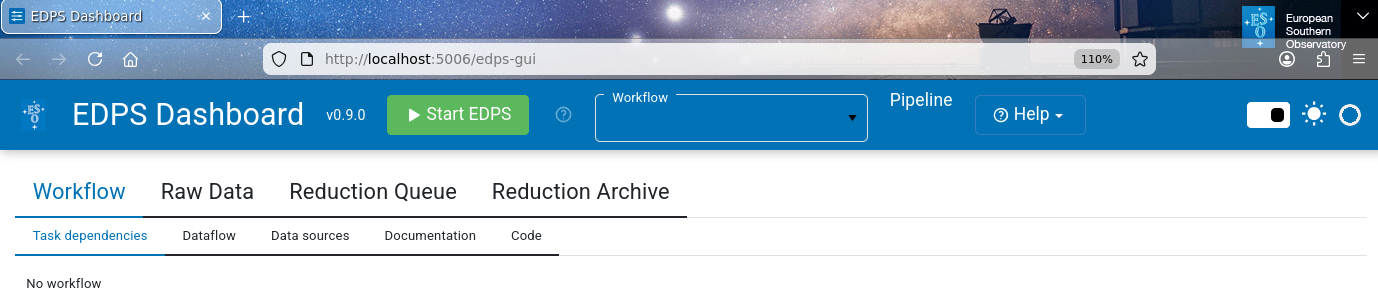
\includegraphics[width=0.9\textwidth]{figures/gui.jpg}
\caption{The \edpsgui\ dashboard (Graphic User Interface). At this stage, \edps\
has not been started yet and no workflow has been selected.}
\label{fig:gui}
\end{figure}

At the top of the Dashboard, near the {\tt Start/Stop EDPS} buttons there
is the {\bf Workflow} selection menu, which allows to load the desired
workflow. The available workflows depend on the pipelines installed in
your system.

The {\tt Help} drop-down menu contains version information, reference,
and the {\bf Settings} menu, which allows to configure several
\edps\ behaviors, such as links to data-storage directories, and the
parallelization.  It is described in detail in Section
\ref{sec:settings}. Note that it is possible to change the
settings only if \edps\ has not been started yet.

There are 4 tabs in the main dashboard window, they are:

\begin{itemize}
\item {\bf Workflow}. It gives information on the workflow, the graphic
  layout, a description of the type of data and access to the workflow
  code. It is described in detail in Section
  \verb|[The **Workflow** tab](#workflow)|.

\item {\bf Raw Data}. It allows to specify the input data, the preferences
  for association calibrations, and to create datasets to be reduced. It
  is described in Section
  \verb|[The **Raw Data** tab](#raw_data)|.

\item {\bf Reduction Queue}. It starts the data reduction. It is described in
  Section
  \verb|[The **Reduction Queue** tab](#reduction_queue)|.

\item {\bf Reduction Archive}. It gives access to previously archived data
  reduction and final products. It is described in Section
  \verb|[The **Reduction Archive** tab](#reduction_archive)|.
\end{itemize}

At the bottom of the dashboard, the graphic representation of the
selected workflow is visible.
% {numref}`fig-workflow-tab` shows the EDPS dashboard with the FORS spectroscopic workflow loaded.




\subsection{Settings}
\label{sec:settings}
\end{document}

```{include} settings_.md
```

---
Go to [top](#top)

Go to EDPS-GUI documentation [index](../edpsgui/index)

<a name="workflow"></a>

## The **Workflow** tab.


```{include} workflow_.md
```
---
Go to [top](#top)

Go to the EDPS-GUI documentation [index](../edpsgui/index)

<a name="raw_data"></a>
## The **Raw Data** tab.


```{include} raw_data_.md
```

---
Go to [top](#top)

Go to the EDPS-GUI documentation [index](../edpsgui/index)

<a name="reduction_queue"></a>
## The **Reduction Queue** tab.

```{include} reduction_queue_.md
```

---
Go to [top](#top)

Go to the EDPS-GUI documentation [index](../edpsgui/index)


<a name="reduction_archive"></a>
## The **Reduction Archive** tab.

All the products (final and intermediate) of all reduced configuration for all datasets are saved into
the EDPS_data directory. In addition, EDPS offers the possibility to "archive" a desired reduction (e.g., the one
that gives the best results) by "exporting" only the final reduction products into another location.

Select the desired reduced configurations and press the "Archive button". This configuration disappears from the
Reduction Queue and appear in the tab "Reduction Archive".

The content of the "Reduction Archive", e.g. the list of archived reductions, can be inspected by pressing the
**Reduction Archive" tab.

   ````{figure} figures/export1.jpg
   :alt: archive
   :name: archive
   ```` 

Each configuration and its jobs can be inspected, unarchived and eventually deleted.
In order to copy the final products into a desired location, press the Export button. A window will appear
allowing 
 - to select all or just the last configuration for the selected datasets  
 - to specify a directory where to save the files. A check is done 

Press **Export** to save the files.. 
The types of files to copy depend on each workflow. Typically, only most important files of the 
scientific tasks are saved. Other files can be found in the EDPS_data directory.
The operation can take several minutes, depending on the sizes of the files.
The default structure is `<dataset_name>/<reduction_time_stamp>/<category>.fits`.

   ````{figure} figures/export2.jpg
   :alt: archive2
   :name: archive2
   ````  
---
Go to [top](#top)

Go to the EDPS-GUI documentation [index](../edpsgui/index)

